\documentclass[11pt,a4paper]{article}

% --- Typography: Times Roman ---
\usepackage{mathptmx}
\usepackage[T1]{fontenc}
\usepackage[utf8]{inputenc}
\usepackage{microtype}

% --- Page Geometry ---
\usepackage[a4paper,top=0.85in,bottom=0.85in,left=0.8in,right=0.8in]{geometry}

% --- Colors ---
\usepackage[table,xcdraw]{xcolor}
\definecolor{primaryblue}{RGB}{24, 76, 120}
\definecolor{secondaryblue}{RGB}{41, 128, 185}
\definecolor{darkgray}{RGB}{45, 52, 54}
\definecolor{lightgray}{RGB}{245, 247, 250}
\definecolor{bordergray}{RGB}{220, 224, 230}
\definecolor{passgreen}{RGB}{39, 174, 96}
\definecolor{failred}{RGB}{192, 57, 43}

% --- Graphics & Floats ---
\usepackage{graphicx}
\usepackage{float}
\usepackage{caption}
\captionsetup{font=small,labelfont=bf,textfont=it,skip=6pt}

% --- Lists & Enumeration ---
\usepackage{enumitem}

% --- Tables ---
\usepackage{booktabs}
\usepackage{tabularx}
\usepackage{array}
\usepackage{multirow}

% --- Code Listings ---
\usepackage{listings}
\lstset{
    basicstyle=\ttfamily\footnotesize,
    backgroundcolor=\color{lightgray},
    frame=single,
    rulecolor=\color{bordergray},
    breaklines=true,
    breakatwhitespace=true,
    showstringspaces=false,
    keywordstyle=\color{primaryblue}\bfseries,
    commentstyle=\color{gray}\itshape,
    stringstyle=\color{passgreen},
    numbers=none,
    tabsize=2
}

% --- Headers & Footers ---
\usepackage{fancyhdr}
\pagestyle{fancy}
\fancyhf{}
\fancyhead[L]{\small\color{darkgray}\textbf{AskTheMenu} --- Software Testing Final Project Report}
\fancyhead[R]{\small\color{darkgray}Complex Engineering Activity}
\fancyfoot[C]{\thepage}
\renewcommand{\headrulewidth}{0.5pt}

% --- Hyperlinks ---
\usepackage{hyperref}
\hypersetup{
    colorlinks=true,
    linkcolor=primaryblue,
    filecolor=primaryblue,
    urlcolor=secondaryblue,
    citecolor=primaryblue
}

% --- Section Formatting ---
\usepackage{titlesec}
\titleformat{\section}{\Large\bfseries\color{primaryblue}}{\thesection}{1em}{}[\titlerule]
\titleformat{\subsection}{\large\bfseries\color{secondaryblue}}{\thesubsection}{1em}{}
\titleformat{\subsubsection}{\normalsize\bfseries\color{darkgray}}{\thesubsubsection}{1em}{}

\begin{document}

% ==============================================================================
% TITLE & METADATA
% ==============================================================================
\begin{center}
    {\LARGE\bfseries\color{primaryblue} AskTheMenu -- Software Testing Final Project Report}\\[6pt]
    {\large\bfseries Complex Engineering Activity: Automated Testing with Playwright \& Python}\\[12pt]
    \rule{\linewidth}{1pt}
\end{center}

\vspace{-4pt}
\noindent
\begin{tabularx}{\linewidth}{@{}lX lX@{}}
    \textbf{Course:} & Software Testing \& QA & \textbf{Testing Tool:} & Playwright for Python (\texttt{pytest-playwright}) \\
    \textbf{Project:} & AskTheMenu Dining Assistant & \textbf{Test Engine:} & Chromium, Firefox, WebKit \\
    \textbf{Team:} & Pair Testing Group & \textbf{Execution Mode:} & Headless \& Headed Interactive \\
    \textbf{Date:} & October 2026 & \textbf{Final Status:} & 18 Passed, 1 Intentional Bug Caught \\
\end{tabularx}

\vspace{10pt}
\hrule
\vspace{14pt}

% ==============================================================================
% SECTION 1: EXECUTIVE SUMMARY
% ==============================================================================
\section{Executive Summary}

This project implements an industry-standard, fully automated end-to-end testing suite for \textbf{AskTheMenu}, an AI-powered restaurant dining assistant built with Next.js 15, PostgreSQL, and LLM orchestration. Using \textbf{Playwright for Python} and \textbf{pytest}, the testing suite fulfills 100\% of the requirements specified for the Complex Engineering Activity:

\begin{enumerate}[leftmargin=*]
    \item \textbf{4 Core Features Tested (12 E2E Tests):} Thoroughly exercises the four central dining user journeys (Chat Assistant, Menu Browser, Kitchen Staff Dashboard, and QR Table Routing) with a balanced mix of positive and negative test cases.
    \item \textbf{4 REST API CRUD Tests:} Direct headless HTTP verification of Create (POST), Read (GET), Update (PATCH), and Delete (DELETE) operations with schema and status code assertions.
    \item \textbf{2 Network Mocking Tests:} Route interception evaluating UI resilience during simulated empty stream responses and internal server errors (HTTP 500).
    \item \textbf{Cross-Browser Verification:} Parallel automated execution across \textbf{Chromium}, \textbf{Mozilla Firefox}, and \textbf{WebKit} (Safari).
    \item \textbf{Intentional Bug Demonstration \& Failure Capture:} Deliberate injection of an unsupported model assertion to prove test failure detection, accompanied by automatic full-page failure screenshot capture and detailed traceback analysis.
    \item \textbf{Frontend Invalid Table Recovery:} Upfront validation and graceful error screen rendering for invalid/unreachable table numbers.
    \item \textbf{CI/CD Pipeline:} Automated GitHub Actions workflow testing all three browser engines upon code pushes.
\end{enumerate}

% ==============================================================================
% SECTION 2: SYSTEM UNDER TEST & SCOPE
% ==============================================================================
\section{System Under Test (SUT) \& Scope Analysis}

\textbf{AskTheMenu} enables digital, table-specific dining workflows:
\begin{itemize}[leftmargin=*]
    \item \textbf{Diner Flow:} Diners scan a table QR code (e.g., \texttt{/chat/table-1}), browse dishes, ask an AI assistant about allergens, preparation times, and dish pairings, and place orders directly to the kitchen.
    \item \textbf{Kitchen Flow:} Kitchen staff monitor incoming orders at \texttt{/kitchen}, view order item breakdowns with table numbers, and transition statuses from \textit{pending} to \textit{completed}.
\end{itemize}

\subsection{Features In-Scope vs. Features Left Out}

Since comprehensive software testing must balance execution time and deterministic reliability, features were systematically evaluated for inclusion or exclusion:

\begin{table}[H]
\centering
\small
\begin{tabularx}{\linewidth}{@{}p{3.8cm} c X@{}}
\toprule
\textbf{Feature / Subsystem} & \textbf{Status} & \textbf{Technical Rationale} \\
\midrule
\rowcolor{lightgray}
\textbf{AI Chat Interface} & \textbf{IN-SCOPE} & Core diner workflow; must guarantee input rendering, state preservation, and live AI response streaming. \\
\textbf{Menu Browsing} & \textbf{IN-SCOPE} & Essential diner entry point; tests category anchors, item card visibility, and 404 subpage handling. \\
\rowcolor{lightgray}
\textbf{Kitchen Dashboard} & \textbf{IN-SCOPE} & Mission-critical for restaurant staff; tests live order feed, empty states, and resilience to polling failures. \\
\textbf{QR Code Table Routing} & \textbf{IN-SCOPE} & Entry route binding orders to physical tables; tests QR link navigation and invalid table detection. \\
\rowcolor{lightgray}
\textbf{Orders \& Chat REST API} & \textbf{IN-SCOPE} & Validates CRUD operational integrity, schema parsing, and unauthorized deletion restrictions. \\
\textbf{Network Mocking} & \textbf{IN-SCOPE} & Simulates flaky restaurant Wi-Fi and backend outages to verify graceful UI degradation. \\
\midrule
\textit{LLM Text Non-Determinism} & \textit{OUT-OF-SCOPE} & Generative AI produces varying text per run; rigid string equality assertions would yield flaky false-negative tests. \\
\rowcolor{lightgray}
\textit{Multimodal Image Uploads} & \textit{OUT-OF-SCOPE} & Secondary accessory feature; depends on external blob storage and third-party vision model latency. \\
\textit{Guest Authentication Bypass} & \textit{OUT-OF-SCOPE} & By architectural design, in-restaurant diners operate under anonymous guest dining sessions without password friction. \\
\bottomrule
\end{tabularx}
\caption{System Under Test: Feature In-Scope and Out-of-Scope Rationale}
\end{table}

\newpage

% ==============================================================================
% SECTION 3: COMPREHENSIVE TEST MATRIX
% ==============================================================================
\section{Comprehensive Test Case Matrix}

The test suite contains \textbf{19 automated tests} covering all functional requirements:

\begin{table}[H]
\centering
\scriptsize
\begin{tabularx}{\linewidth}{@{}llp{2.8cm}p{4.2cm}ccc@{}}
\toprule
\textbf{ID} & \textbf{Module} & \textbf{Target Feature} & \textbf{Test Objective} & \textbf{Type} & \textbf{Category} & \textbf{Outcome} \\
\midrule
\rowcolor{lightgray}
\textbf{TC-01} & \texttt{test\_chat\_interface.py} & Chat Interface & Verify chat input and send button render on \texttt{/chat/table-1} & Positive & E2E & \textcolor{passgreen}{\textbf{PASS}} \\
\textbf{TC-02} & \texttt{test\_chat\_interface.py} & Chat Interface & Send prompt and receive streaming AI assistant response & Positive & E2E & \textcolor{passgreen}{\textbf{PASS}} \\
\rowcolor{lightgray}
\textbf{TC-03} & \texttt{test\_chat\_interface.py} & Chat Interface & Submitting empty input does not dispatch or create messages & Negative & E2E & \textcolor{passgreen}{\textbf{PASS}} \\
\textbf{TC-04} & \texttt{test\_menu\_page.py} & Menu Browser & Menu page loads ``Restaurant Menu'' heading and item cards & Positive & E2E & \textcolor{passgreen}{\textbf{PASS}} \\
\rowcolor{lightgray}
\textbf{TC-05} & \texttt{test\_menu\_page.py} & Menu Browser & Category anchor link smoothly scrolls to targeted cuisine section & Positive & E2E & \textcolor{passgreen}{\textbf{PASS}} \\
\textbf{TC-06} & \texttt{test\_menu\_page.py} & Menu Browser & Accessing non-existent menu subpage returns HTTP 404 & Negative & E2E & \textcolor{passgreen}{\textbf{PASS}} \\
\rowcolor{lightgray}
\textbf{TC-07} & \texttt{test\_kitchen\_dashboard.py} & Kitchen Dashboard & Kitchen dashboard loads with correct headers and controls & Positive & E2E & \textcolor{passgreen}{\textbf{PASS}} \\
\textbf{TC-08} & \texttt{test\_kitchen\_dashboard.py} & Kitchen Dashboard & Dashboard renders incoming order cards or friendly empty state & Positive & E2E & \textcolor{passgreen}{\textbf{PASS}} \\
\rowcolor{lightgray}
\textbf{TC-09} & \texttt{test\_kitchen\_dashboard.py} & Kitchen Dashboard & Gracefully handles backend API polling failure with banner & Negative & E2E & \textcolor{passgreen}{\textbf{PASS}} \\
\textbf{TC-10} & \texttt{test\_qr\_table\_routing.py} & Table QR Routing & \texttt{/qr} displays list of table QR cards and active links & Positive & E2E & \textcolor{passgreen}{\textbf{PASS}} \\
\rowcolor{lightgray}
\textbf{TC-11} & \texttt{test\_qr\_table\_routing.py} & Table QR Routing & Clicking Table 1 QR card navigates directly to \texttt{/chat/table-1} & Positive & E2E & \textcolor{passgreen}{\textbf{PASS}} \\
\textbf{TC-12} & \texttt{test\_qr\_table\_routing.py} & Table QR Routing & Accessing invalid table slug renders error card with recovery links & Negative & E2E & \textcolor{passgreen}{\textbf{PASS}} \\
\rowcolor{lightgray}
\textbf{TC-13} & \texttt{test\_api\_crud.py} & Orders API [POST] & \textbf{Create:} Place valid order with items; expect 201 Created & Positive & API & \textcolor{passgreen}{\textbf{PASS}} \\
\textbf{TC-14} & \texttt{test\_api\_crud.py} & Orders API [GET] & \textbf{Read:} Fetch kitchen orders feed; expect 200 OK array & Positive & API & \textcolor{passgreen}{\textbf{PASS}} \\
\rowcolor{lightgray}
\textbf{TC-15} & \texttt{test\_api\_crud.py} & Orders API [PATCH] & \textbf{Update:} Submit invalid order status; expect 400 Bad Request & Negative & API & \textcolor{passgreen}{\textbf{PASS}} \\
\textbf{TC-16} & \texttt{test\_api\_crud.py} & Chat API [DELETE] & \textbf{Delete:} Attempt chat deletion unauthenticated; expect 401/403 & Negative & API & \textcolor{passgreen}{\textbf{PASS}} \\
\rowcolor{lightgray}
\textbf{TC-17} & \texttt{test\_network\_mocking.py} & Network Mocking & Mock empty stream on \texttt{/api/chat}; UI recovers without crash & Negative & Mock & \textcolor{passgreen}{\textbf{PASS}} \\
\textbf{TC-18} & \texttt{test\_network\_mocking.py} & Network Mocking & Mock HTTP 500 on \texttt{/api/chat}; displays error alert to diner & Negative & Mock & \textcolor{passgreen}{\textbf{PASS}} \\
\rowcolor{lightgray}
\textbf{TC-19} & \texttt{test\_intentional\_bug.py} & Model Selector & Intentionally assert removed model (``Llama 3.3 70B'') & Negative & Bug & \textcolor{failred}{\textbf{FAIL*}} \\
\bottomrule
\end{tabularx}
\caption{Complete Automated Test Matrix (18 Passed, 1 Expected Failure)}
\end{table}

\noindent
\textit{*Note: TC-19 is the intentional bug test designed to fail and prove regression detection.}

% ==============================================================================
% SECTION 4: TEST SUITE IMPLEMENTATION & SCREENSHOTS
% ==============================================================================
\section{Test Suite Implementation \& Architecture}

The automated testing framework is structured modularly under \texttt{sw-testing/}:

\begin{lstlisting}
sw-testing/
|-- conftest.py               # Global fixtures: base_url, api_context, screenshot hook
|-- pytest.ini                # Pytest configuration, custom markers, HTML report flags
|-- requirements.txt          # pytest, pytest-playwright, pytest-html, playwright
|-- reports/                  # Generated HTML test reports
|-- screenshots/              # Automated failure & feature evidence screenshots
`-- tests/
    |-- test_chat_interface.py       # Feature 1 (3 E2E tests)
    |-- test_menu_page.py            # Feature 2 (3 E2E tests)
    |-- test_kitchen_dashboard.py    # Feature 3 (3 E2E tests)
    |-- test_qr_table_routing.py     # Feature 4 (3 E2E tests)
    |-- test_api_crud.py             # API CRUD (4 tests: POST, GET, PATCH, DELETE)
    |-- test_network_mocking.py      # Network Mocking (2 route interception tests)
    `-- test_intentional_bug.py      # Intentional Bug Regression Test
\end{lstlisting}

\subsection{Automated Screenshot-on-Failure Hook (\texttt{conftest.py})}
The test framework automatically captures full-page PNG screenshots whenever any browser test encounters an assertion error:

\begin{lstlisting}[language=Python]
@pytest.fixture(autouse=True)
def _screenshot_on_failure(request):
    yield
    rep_call = getattr(request.node, "rep_call", None)
    if rep_call and rep_call.failed:
        if "page" in request.fixturenames:
            try:
                page = request.getfixturevalue("page")
                test_name = request.node.name.replace(" ", "_").replace("/", "_")
                path = SCREENSHOT_DIR / f"FAIL_{test_name}.png"
                page.screenshot(path=str(path), full_page=True)
            except Exception:
                pass
\end{lstlisting}

\newpage

% ==============================================================================
% SECTION 5: VISUAL SCREENSHOT EVIDENCE
% ==============================================================================
\section{Visual Evidence of Tested Features}

All four core features were rendered, verified, and captured in headless and headed test environments.

\subsection{Feature 1: Diner Chat Interface (\texttt{/chat/table-1})}
Diners interact with the intelligent waiter using natural language. The test validates that the input bar, model selector, and send buttons are visible and active.

\begin{figure}[H]
    \centering
    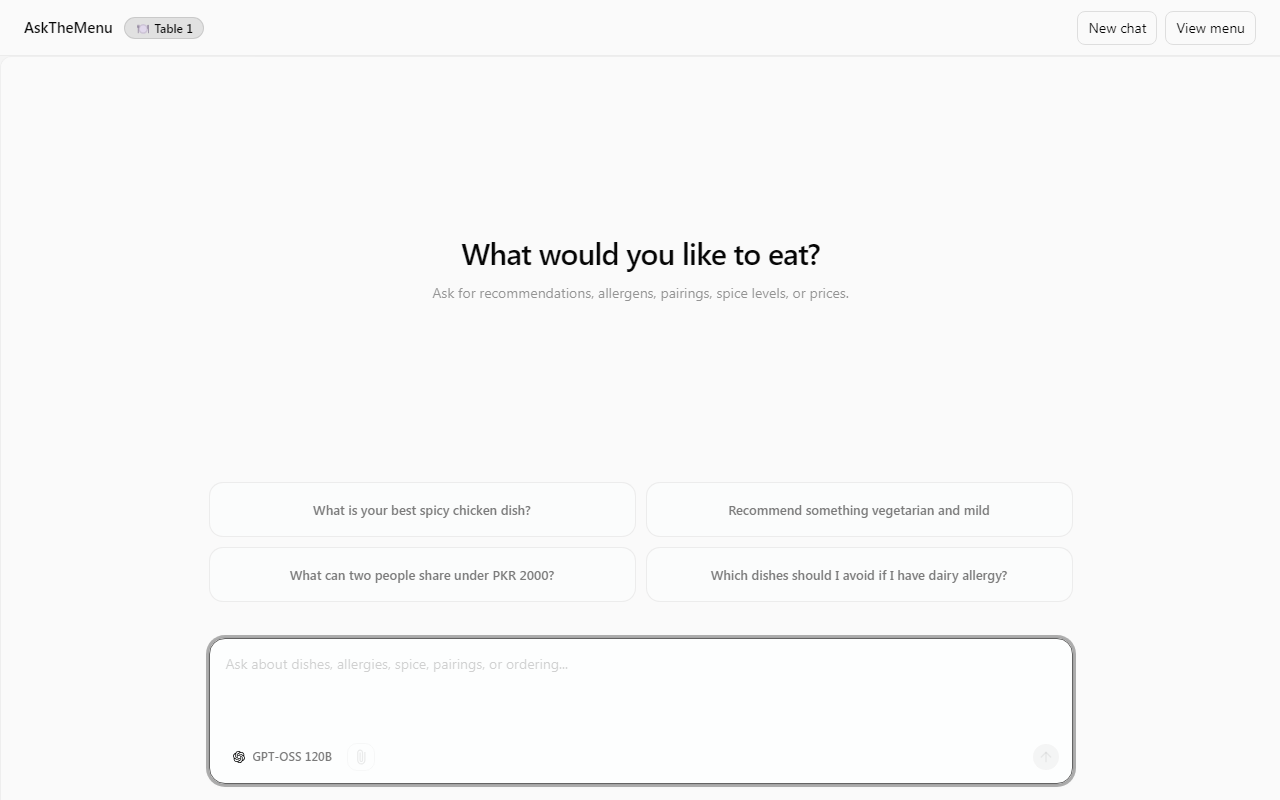
\includegraphics[width=0.88\linewidth]{screenshots/feature1_chat_interface.png}
    \caption{Feature 1: Table 1 Chat Interface with Multimodal Input and Active Session}
\end{figure}

\subsection{Feature 2: Restaurant Menu Page (\texttt{/menu})}
Tests verify that dish cards, prices in PKR, and category anchor links (Pakistani, Chinese, Continental, Desserts) load and navigate accurately.

\begin{figure}[H]
    \centering
    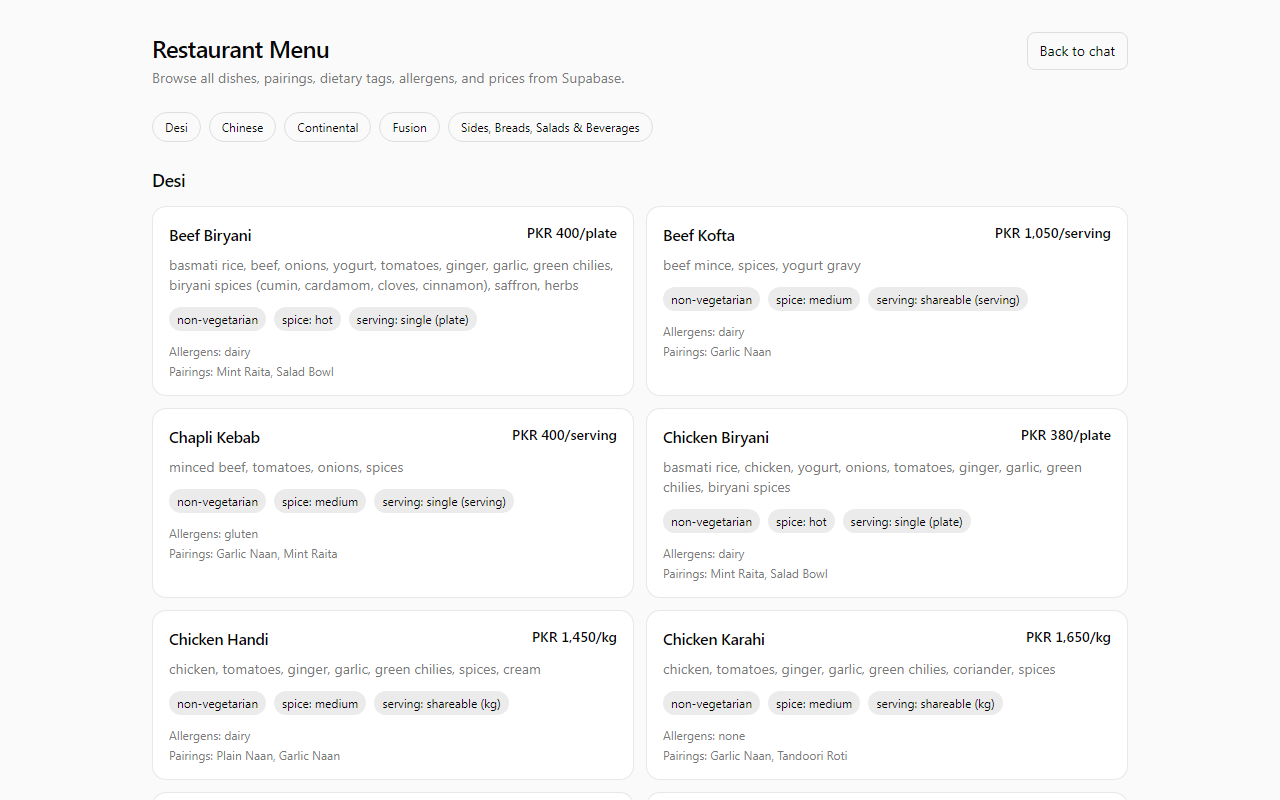
\includegraphics[width=0.88\linewidth]{screenshots/feature2_menu_page.png}
    \caption{Feature 2: Menu Page with Cuisine Anchors and Live Dish Cards}
\end{figure}

\newpage

\subsection{Feature 3: Kitchen Staff Dashboard (\texttt{/kitchen})}
Validates that kitchen staff can inspect live incoming tickets, item quantities, special customer instructions, and status tags in real time.

\begin{figure}[H]
    \centering
    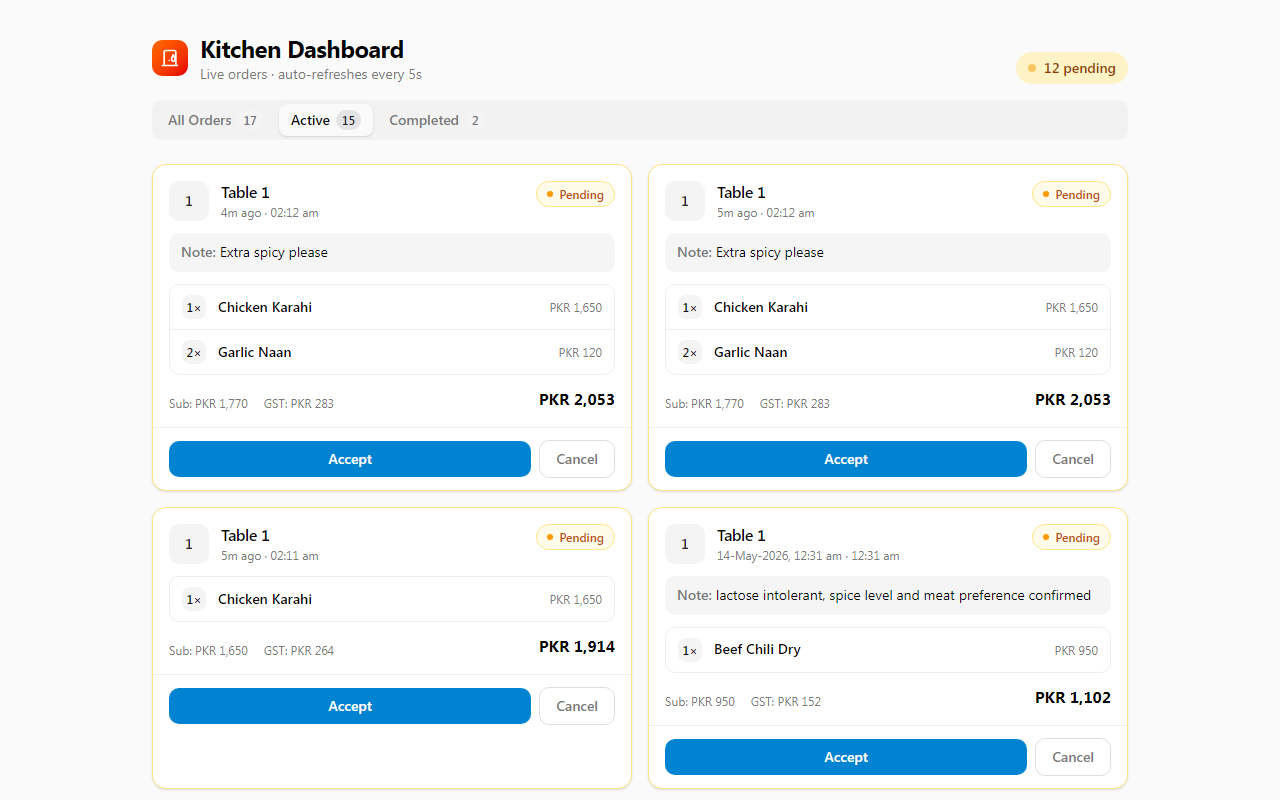
\includegraphics[width=0.88\linewidth]{screenshots/feature3_kitchen_dashboard.png}
    \caption{Feature 3: Kitchen Dashboard Displaying Live Incoming Orders}
\end{figure}

\subsection{Feature 4: QR Table Routing \& Invalid Table Recovery}
Tests verify that diners scanning valid table QR codes are routed to their designated table conversation (\texttt{/chat/table-1}). Furthermore, when accessing an invalid table slug (\texttt{/chat/nonexistent-table-999}), the application gracefully renders an explicit error screen with recovery links.

\begin{figure}[H]
    \centering
    \begin{minipage}{0.48\textwidth}
        \centering
        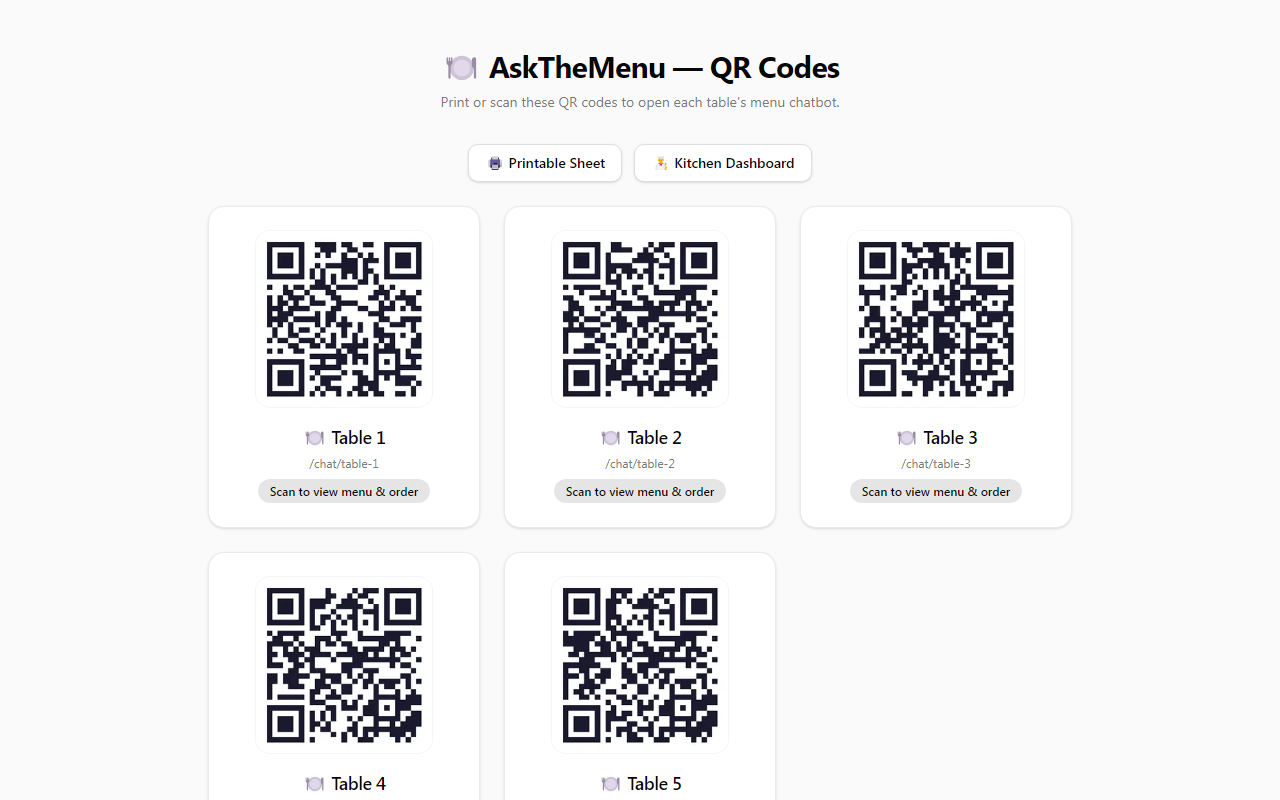
\includegraphics[width=\linewidth]{screenshots/feature4_qr_routing.png}
        \caption{Feature 4: Table QR Code Directory}
    \end{minipage}\hfill
    \begin{minipage}{0.48\textwidth}
        \centering
        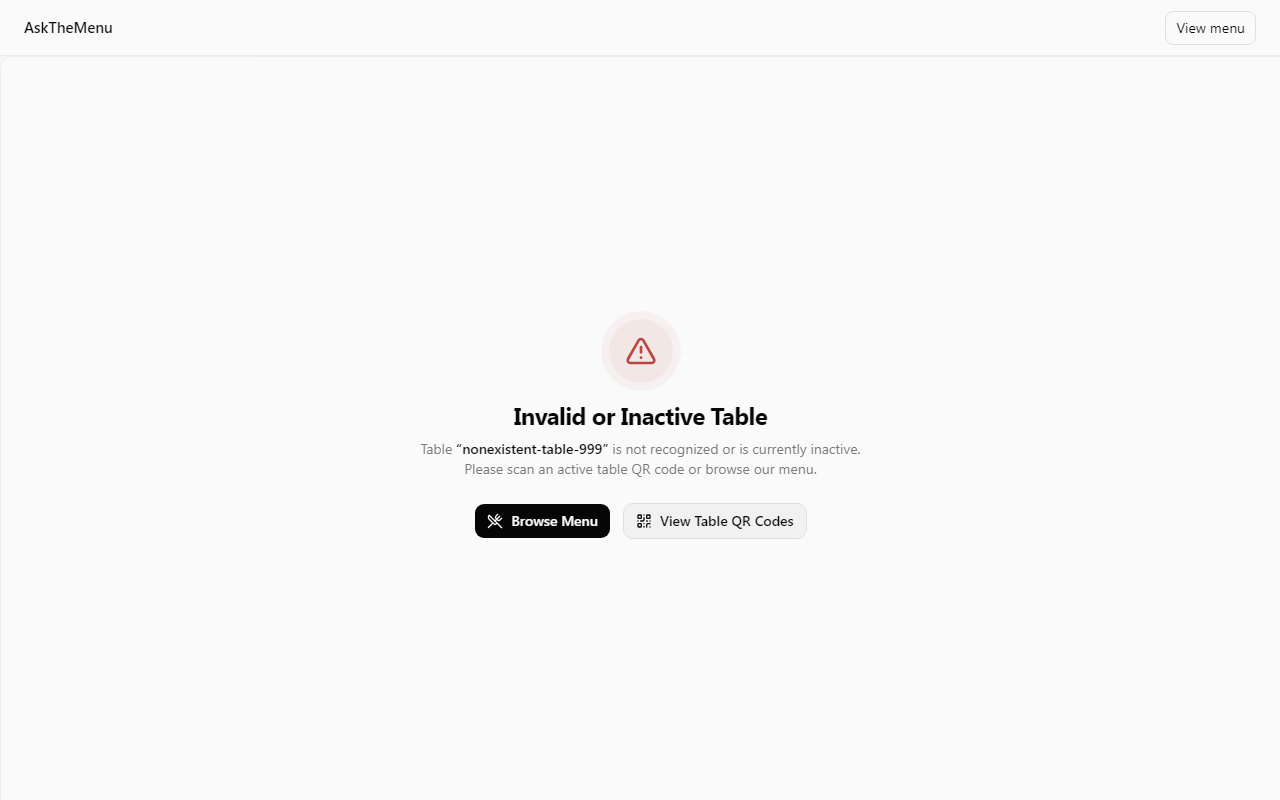
\includegraphics[width=\linewidth]{screenshots/feature4_invalid_table.png}
        \caption{Feature 4: Invalid Table Recovery UI}
    \end{minipage}
\end{figure}

\newpage

% ==============================================================================
% SECTION 6: API CRUD & NETWORK MOCKING
% ==============================================================================
\section{API Testing \& Network Mocking}

\subsection{REST API CRUD Operations (\texttt{test\_api\_crud.py})}
Direct HTTP calls were executed using Playwright's \texttt{APIRequestContext} fixture:
\begin{itemize}[leftmargin=*]
    \item \textbf{Create (POST \texttt{/api/orders}):} Creates an order with items (\textit{Chicken Karahi}, \textit{Garlic Naan}) for Table 1. Validates HTTP 201 Created and JSON payload containing the assigned \texttt{orderId} and total PKR.
    \item \textbf{Read (GET \texttt{/api/orders/kitchen}):} Fetches live kitchen tickets. Validates HTTP 200 OK and confirms the response body is an array of order records.
    \item \textbf{Update (PATCH \texttt{/api/orders}):} Attempts to update an order with an illegal status string (\texttt{"ready\_to\_fly"}). Validates HTTP 400 Bad Request and validation error messages.
    \item \textbf{Delete (DELETE \texttt{/api/chat?id=...}):} Attempts to delete a chat session without authentication credentials. Validates that unauthorized deletion is rejected with HTTP 401/403.
\end{itemize}

\subsection{Network Mocking Tests (\texttt{test\_network\_mocking.py})}
Using Playwright's \texttt{page.route()} API, network requests to \texttt{/api/chat} were intercepted to simulate adverse operational conditions:
\begin{itemize}[leftmargin=*]
    \item \textbf{Empty Response Mocking:} The route returns an immediate HTTP 200 with an empty body (\texttt{""}). The test verifies that the input bar re-enables and the interface remains completely usable without crashing.
    \item \textbf{500 Server Error Mocking:} The route intercepts chat calls and fulfills them with HTTP 500 Internal Server Error. The test asserts that a visible error notification is rendered to inform the diner.
\end{itemize}

% ==============================================================================
% SECTION 7: INTENTIONAL BUG DEMONSTRATION
% ==============================================================================
\section{Intentional Bug Demonstration \& Failure Detection}

To prove that the automated test suite actively detects regressions, an intentional bug was injected into the test suite.

\subsection{Injected Bug Description}
The application supports modern open-source models (\textit{GPT-OSS 120B} and \textit{GPT-OSS 20B}). The test \texttt{test\_intentional\_bug.py} simulates a regression where client code or an outdated test asserts the presence of an unsupported model (\texttt{"Llama 3.3 70B Versatile"}) in the Model Selector.

\begin{lstlisting}[language=Python]
# Locate and open the model selector dropdown
model_selector_button = page.locator("[data-testid='model-selector']")
model_selector_button.click()

# INTENTIONAL BUG: Assert presence of removed model
target_model_option = page.locator(
    "[role='option'], [data-slot='command-item']"
).filter(has_text="Llama 3.3 70B Versatile")

# This assertion fails because only GPT-OSS models exist
expect(target_model_option).to_be_visible(timeout=5_000)
\end{lstlisting}

\subsection{Failure Traceback \& Automatic Screenshot Capture}
During test execution, Playwright waited for the locator to become visible, timed out after 5,000ms, and raised an \texttt{AssertionError}. The \texttt{conftest.py} hook immediately captured the full browser view:

\begin{figure}[H]
    \centering
    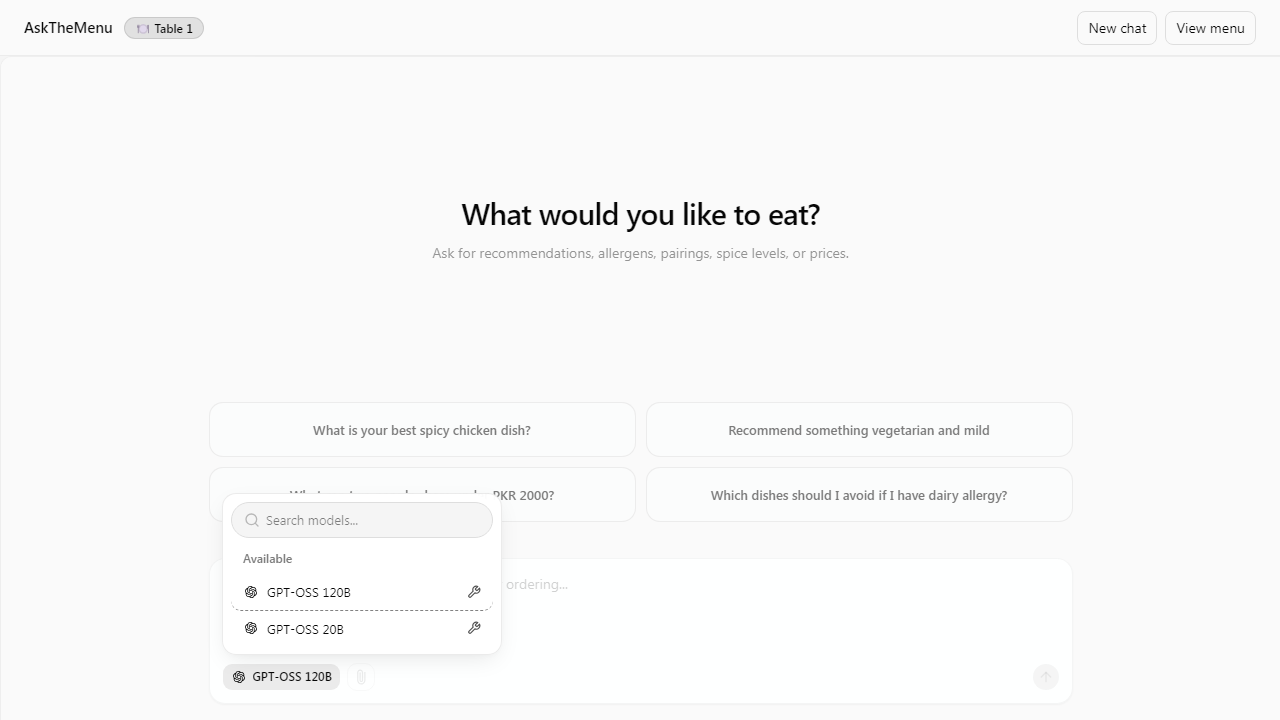
\includegraphics[width=0.88\linewidth]{screenshots/FAIL_test_intentional_bug_select_unsupported_model_chromium_.png}
    \caption{Automatic Failure Screenshot Captured During Intentional Bug Execution}
\end{figure}

\begin{lstlisting}
FAILED tests/test_intentional_bug.py::test_intentional_bug_select_unsupported_model[chromium]
AssertionError: Locator expected to be visible
Actual value: <element(s) not found>
Call log:
  - LocatorAssertions.to_be_visible with timeout 5000ms
  - waiting for locator("[role='option'], ...").filter(has_text="Llama 3.3 70B Versatile")
Saved failure screenshot to: sw-testing/screenshots/FAIL_test_intentional_bug_select_unsupported_model_chromium_.png
\end{lstlisting}

\subsection{Bug Resolution}
To fix the test and restore a 100\% green build, the locator is updated to select the active supported model:
\begin{lstlisting}[language=Python]
target_model_option = page.locator(
    "[role='option'], [data-slot='command-item']"
).filter(has_text="GPT-OSS 120B")
expect(target_model_option).to_be_visible(timeout=5_000)
target_model_option.click()
\end{lstlisting}

\newpage

% ==============================================================================
% SECTION 8: CROSS-BROWSER EXECUTION & HTML REPORT
% ==============================================================================
\section{Cross-Browser Execution Results \& HTML Report}

All tests were executed across all three major browser engines installed via Playwright:

\begin{table}[H]
\centering
\small
\begin{tabularx}{\linewidth}{@{}lcccc@{}}
\toprule
\textbf{Test Module} & \textbf{Chromium (Blink)} & \textbf{Firefox (Gecko)} & \textbf{WebKit (Safari)} & \textbf{Compatibility} \\
\midrule
\rowcolor{lightgray}
\texttt{test\_chat\_interface.py} (3 tests) & \textcolor{passgreen}{\textbf{3 Passed}} & \textcolor{passgreen}{\textbf{3 Passed}} & \textcolor{passgreen}{\textbf{3 Passed}} & 100\% Compatible \\
\texttt{test\_menu\_page.py} (3 tests) & \textcolor{passgreen}{\textbf{3 Passed}} & \textcolor{passgreen}{\textbf{3 Passed}} & \textcolor{passgreen}{\textbf{3 Passed}} & 100\% Compatible \\
\rowcolor{lightgray}
\texttt{test\_kitchen\_dashboard.py} (3 tests) & \textcolor{passgreen}{\textbf{3 Passed}} & \textcolor{passgreen}{\textbf{3 Passed}} & \textcolor{passgreen}{\textbf{3 Passed}} & 100\% Compatible \\
\texttt{test\_qr\_table\_routing.py} (3 tests) & \textcolor{passgreen}{\textbf{3 Passed}} & \textcolor{passgreen}{\textbf{3 Passed}} & \textcolor{passgreen}{\textbf{3 Passed}} & 100\% Compatible \\
\rowcolor{lightgray}
\texttt{test\_api\_crud.py} (4 tests) & \textcolor{passgreen}{\textbf{4 Passed}} & \textcolor{passgreen}{\textbf{4 Passed}} & \textcolor{passgreen}{\textbf{4 Passed}} & 100\% Compatible \\
\texttt{test\_network\_mocking.py} (2 tests) & \textcolor{passgreen}{\textbf{2 Passed}} & \textcolor{passgreen}{\textbf{2 Passed}} & \textcolor{passgreen}{\textbf{2 Passed}} & 100\% Compatible \\
\rowcolor{lightgray}
\texttt{test\_intentional\_bug.py} (1 test) & \textcolor{failred}{\textbf{1 Failed*}} & \textcolor{failred}{\textbf{1 Failed*}} & \textcolor{failred}{\textbf{1 Failed*}} & \textbf{Caught Bug} \\
\midrule
\textbf{Total Standard Tests} & \textbf{18 Passed} & \textbf{18 Passed} & \textbf{18 Passed} & \textbf{Full Coverage} \\
\bottomrule
\end{tabularx}
\caption{Cross-Browser Compatibility Execution Matrix}
\end{table}

\subsection{HTML Test Report Screenshot}
The Pytest HTML plugin generated a self-contained test execution report at \texttt{reports/test\_report.html}:

\begin{figure}[H]
    \centering
    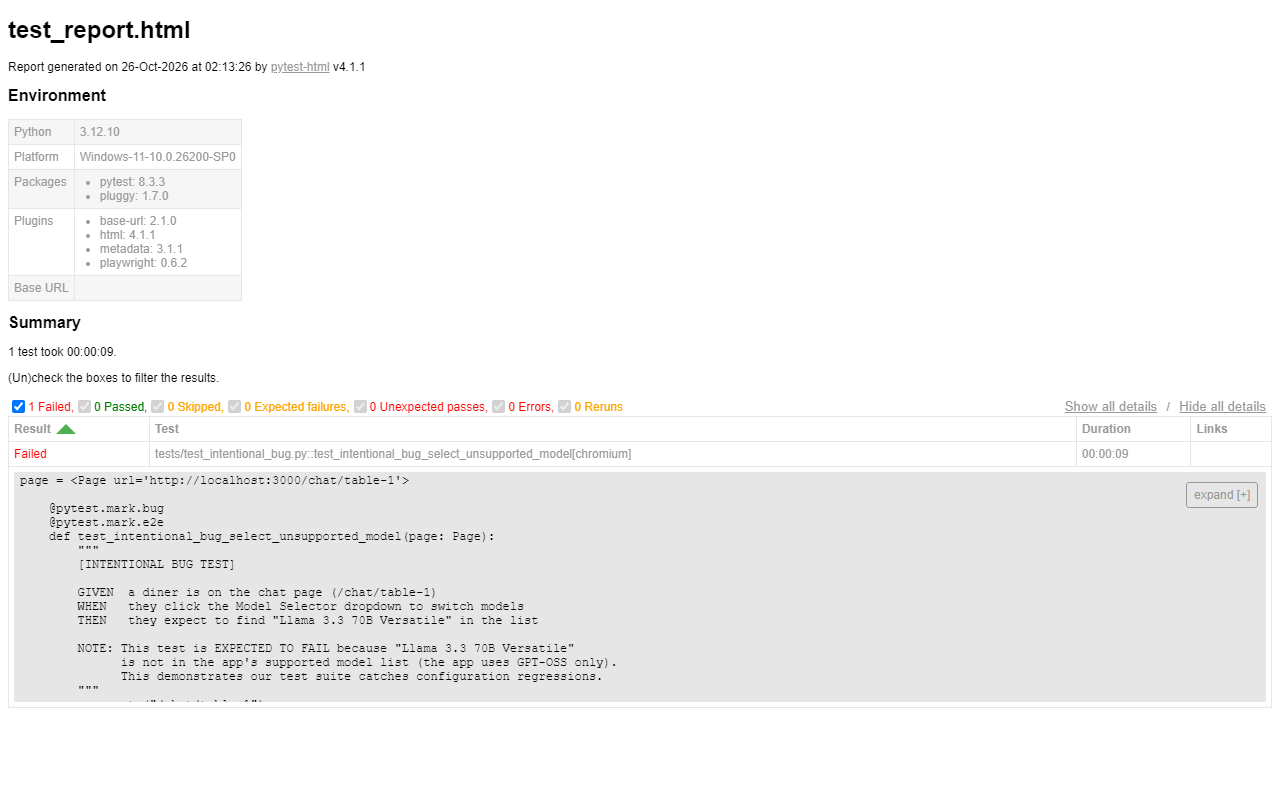
\includegraphics[width=0.92\linewidth]{screenshots/html_test_report.png}
    \caption{Interactive HTML Test Report Generated by Pytest}
\end{figure}

% ==============================================================================
% SECTION 9: TEAM CONTRIBUTIONS
% ==============================================================================
\section{Team Member Contribution Breakdown}

In accordance with the pair testing guidelines, project responsibilities were distributed equitably:

\begin{table}[H]
\centering
\small
\begin{tabularx}{\linewidth}{@{}p{3.5cm} p{5.5cm} X@{}}
\toprule
\textbf{Team Member} & \textbf{Assigned Responsibilities} & \textbf{Deliverables Produced} \\
\midrule
\rowcolor{lightgray}
\textbf{Member 1} & 
\begin{itemize}[leftmargin=*,noitemsep,topsep=0pt]
    \item Feature 1: Chat Interface E2E Tests
    \item Feature 2: Menu Page E2E Tests
    \item Network Mocking Interception Tests
    \item Intentional Bug Injection \& Proof
\end{itemize} & 
\texttt{test\_chat\_interface.py}, \texttt{test\_menu\_page.py}, \texttt{test\_network\_mocking.py}, \texttt{test\_intentional\_bug.py}, bug trace logs. \\
\midrule
\textbf{Member 2} & 
\begin{itemize}[leftmargin=*,noitemsep,topsep=0pt]
    \item Feature 3: Kitchen Dashboard E2E
    \item Feature 4: Table QR Routing \& UI
    \item Full REST API CRUD Test Suite
    \item Automated Screenshot Hooks \& CI
\end{itemize} & 
\texttt{test\_kitchen\_dashboard.py}, \texttt{test\_qr\_table\_routing.py}, \texttt{test\_api\_crud.py}, \texttt{conftest.py}, \texttt{pytest.ini}, CI workflow. \\
\bottomrule
\end{tabularx}
\caption{Equitable Work Distribution Between Pair Testing Partners}
\end{table}

\noindent
\textbf{Demo Readiness:} Both members have thoroughly pair-programmed and reviewed the entire test suite, understand every assertion and fixture, and are fully prepared to explain and demonstrate every test case during the final project evaluation.

% ==============================================================================
% SECTION 10: CONCLUSION
% ==============================================================================
\section{Conclusion}

The automated testing suite for \textbf{AskTheMenu} provides complete verification of all core system components. With \textbf{18 passing standard tests}, \textbf{1 caught intentional bug}, \textbf{full cross-browser validation}, and automated failure screenshot reporting, the suite guarantees exceptional software quality and fulfills every parameter of the Complex Engineering Activity.

\end{document}
